% !TEX root =../thesis.tex
\chapter{Linear interpolation in N-Dimensions}
\label{chap:four}

\lettrine[lines=4]{I}{nterpolation} is one of the most common operations in astronomy. Irregardless if one needs move spectra to a different wavelength grid to coadd them, resampling images to align them or interpolating physical qunatities in N-dimensional fluid dynamics simulation, interpolation plays a central role.
Interpolation can be described as a special case of curve fitting which requires the function to go through all points. 

In one dimension interpolation is relatively easy and there existmultiple methods. The simplest method is nearest-neighbour interpolation in which the interpolation picks the closes neighbour point to thew point to be interpolated.  
Linear interpolation is one of the most common methods of interpolation. The two neighbouring points of the point to be interpolated are found and using their slope and offset the value is interpolated.

There exist more complex interpolation methods like splines that employ polynomials of n-th degree whose first and second derivation need to be the same at the data points. 

Where there exist many methods for interpolation in one dimensional space, the number of options decreases rapidly with the number of dimensions increasing. 
Although the number is decreasing there exist still a number of methods for n-dimensional interpolation, including nearest neighbour interpolation, Radial basis function and delauney triangulation.

We have decided on \deltri and have opted for the QHull-implementation  \citep{Barber96thequickhull} in our case.

The interpolation using \deltri\ has multiple steps to arrive at an  interpolation, which we will describe in the next few sections. First a delauney triangulation is performed on the existing grid. For a point to be interpolated we will need to find the triangle that contains the point. Using this triangle and the barycentric coordinates the actual interpolation is performed. 






\section{Delauney triangulation}
\label{sec:delauney_tri}
A triangulation describes the process of connecting all points in a set with straight lines without any two lines crossing (see Figure \ref{fig:delauney:example}). It is obvious that there many ways for a set to to be triangulated. All triangulations however have the same outer boundary called the convex hull. One special kind of triangulation is the delauney triangulation. The delauney triangulation can be defined a various abstract ways and have intriguing properties. 
One such defintion is that the circum-circle of each triangle must only contain three points. Figure \ref{fig:delauney_illegal}, a simple two dimensional example, shows one \textit{legal} triangulation and one \textit{illegal} triangulation. One can see in the \textit{illegal} triangulation that the the inscribing circles of both triangles contain more than tree points. By doing a simple "\textit{edge-flip}" one arrives at the delauney triangulation. In addition this ensures that the triangulation gives the largest minimum angle for both triangles. 

\deltri\ and convex hulls have a very interesting relation. It is possible construct the \deltri\ in n dimensions from a convex hull of the points projected on paraboloid in n+1 dimensions.
Figure \ref{fig:delauney_projection} shows an example of a \deltri\ in two dimensions constructed from the convex hull in three dimensions. To project the points onto the paraboloid one just square sums the coordinates n dimensions and uses this as the coordinate for the point in n+1 dimensions. 

\begin{figure}[htbp] %  figure placement: here, top, bottom, or page
   \centering
   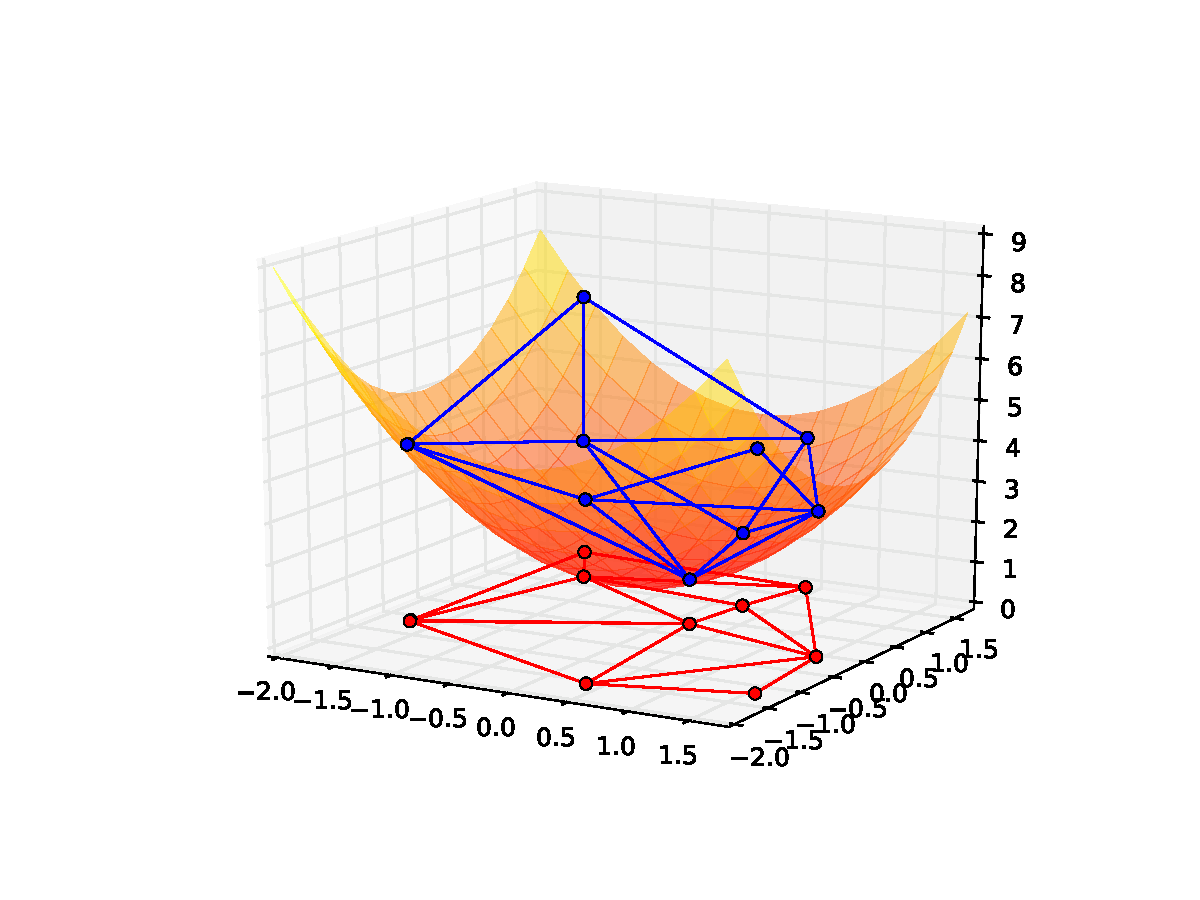
\includegraphics[width=0.49\textwidth]{chapter7/plots/delauney_project_left.pdf} 
   \hspace{-1.5cm}
   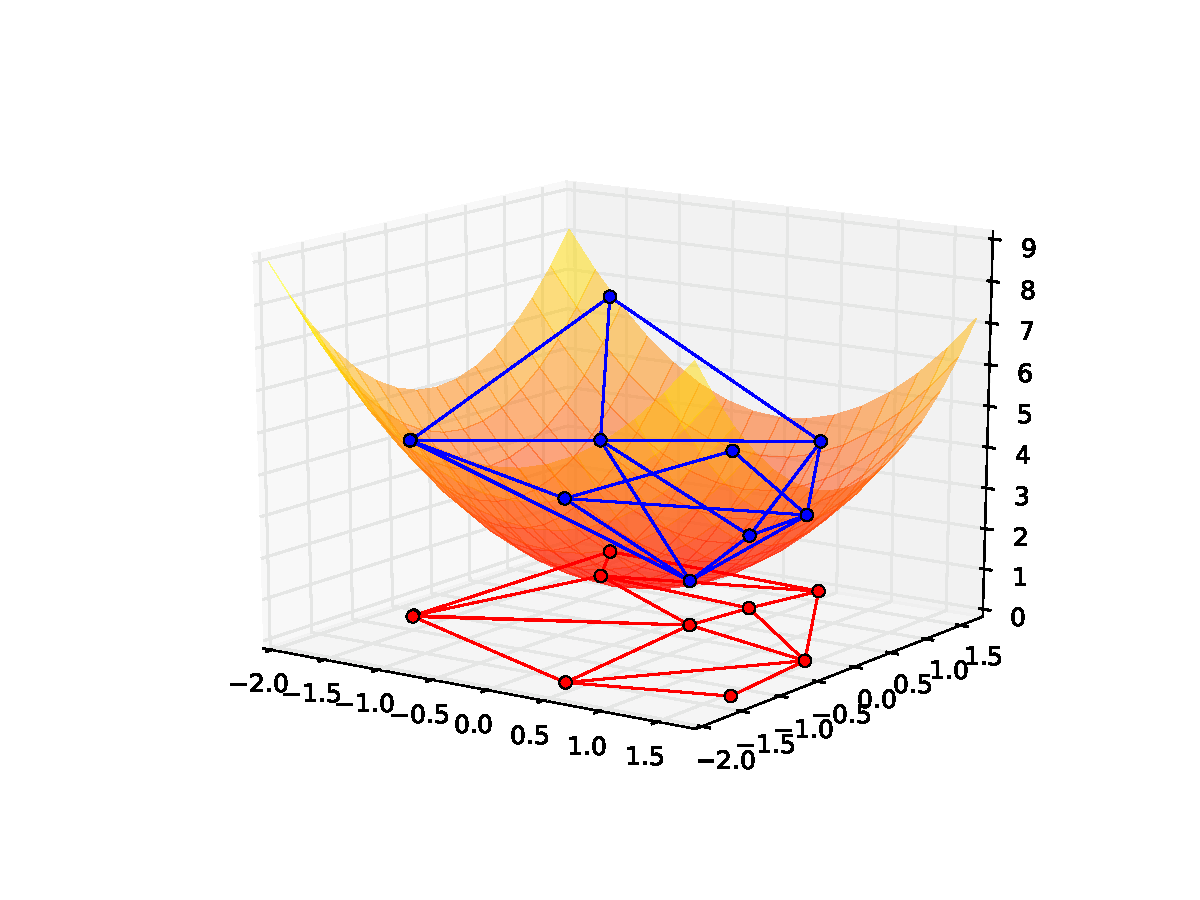
\includegraphics[width=0.49\textwidth]{chapter7/plots/delauney_project_right.pdf} 
   \caption{example caption}
   \label{fig:delauney_projection}
\end{figure}

\section{Convex Hull}

In section \ref{sec:delauney_tri} we have described the relation between the convex hull  and the \deltri. There are multiple ways to construct the convex hull for N points, we will limit ourselves to the description of the Quickhull algorithm. Similar to the Quicksort algorithm it follows the divide and conquer method. 


\begin{figure}[htbp] %  figure placement: here, top, bottom, or page
   \centering
   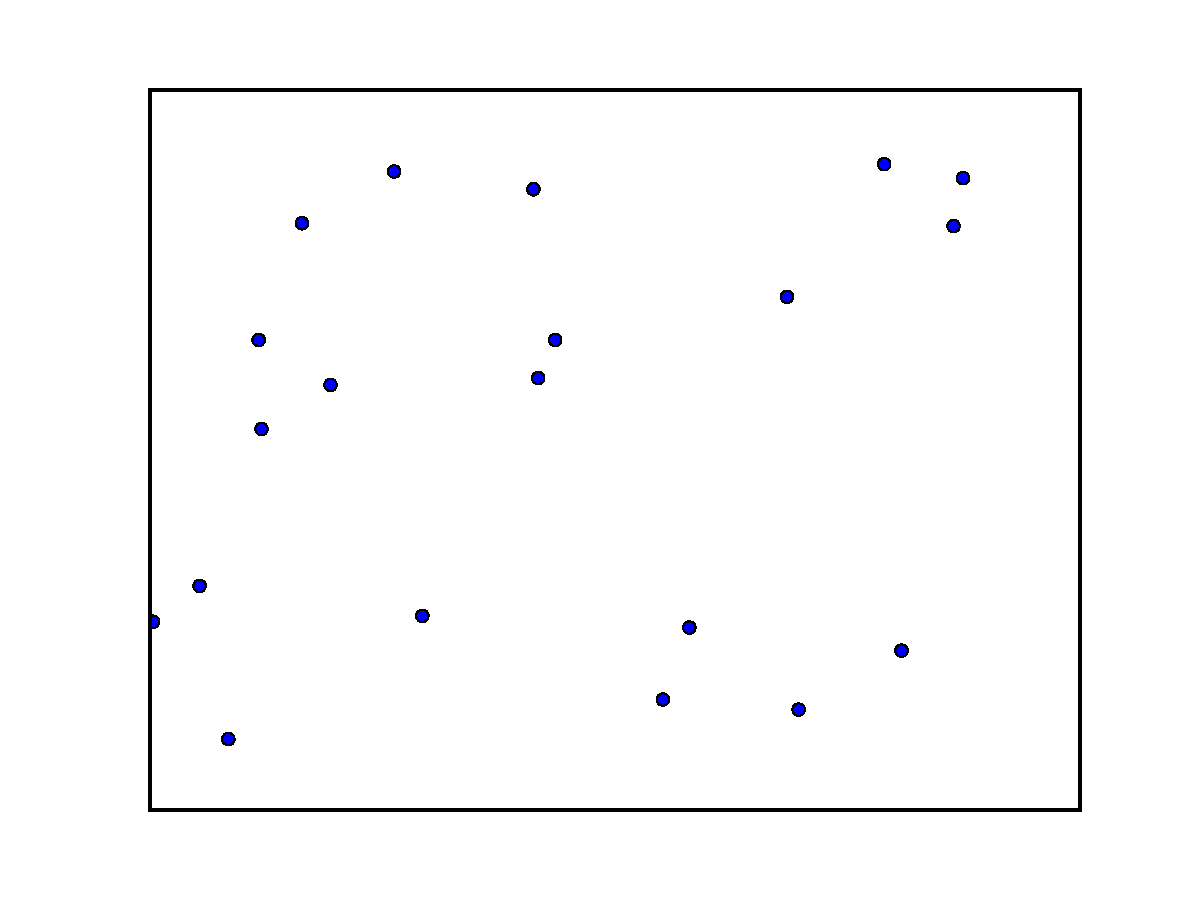
\includegraphics[width=0.49\textwidth]{chapter7/plots/qhull_1.pdf} 
   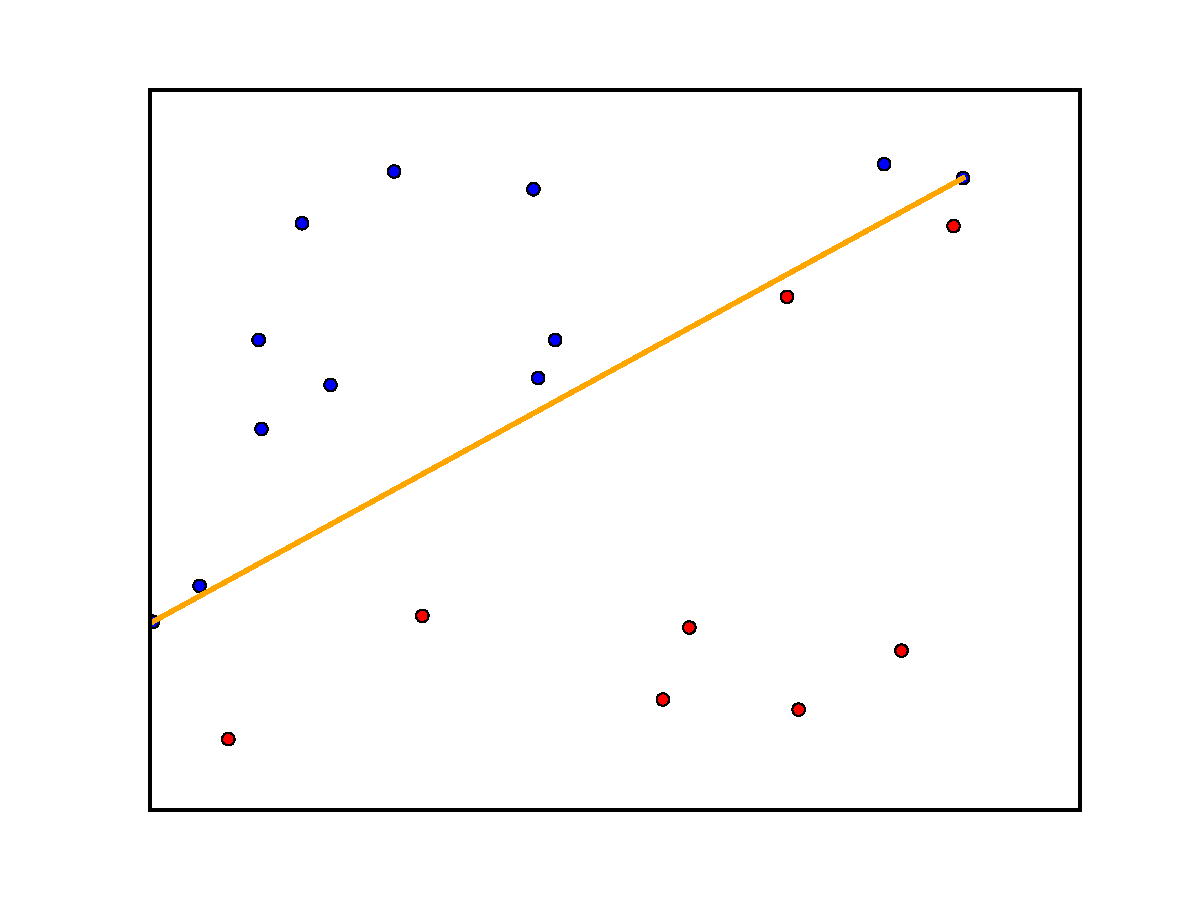
\includegraphics[width=0.49\textwidth]{chapter7/plots/qhull_2.pdf} 
   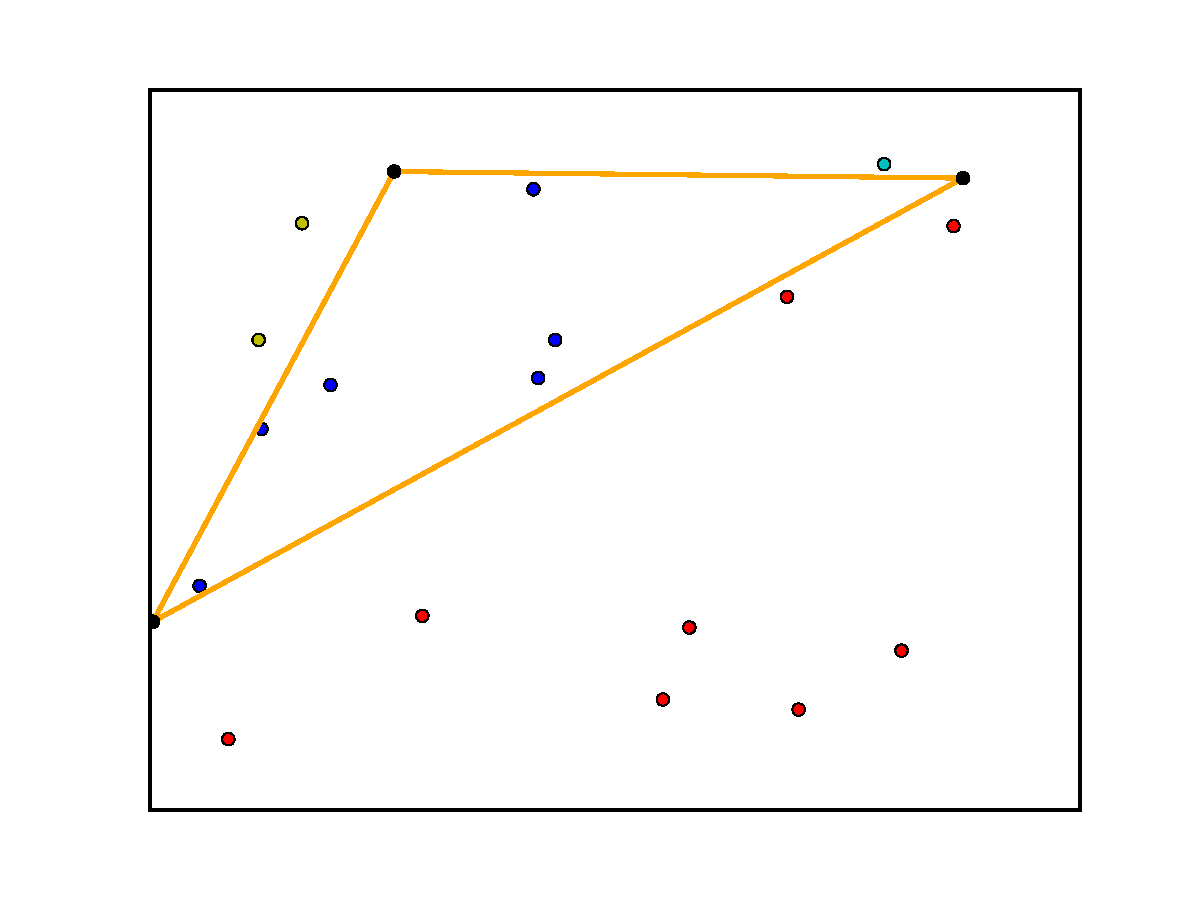
\includegraphics[width=0.49\textwidth]{chapter7/plots/qhull_3.pdf} 
   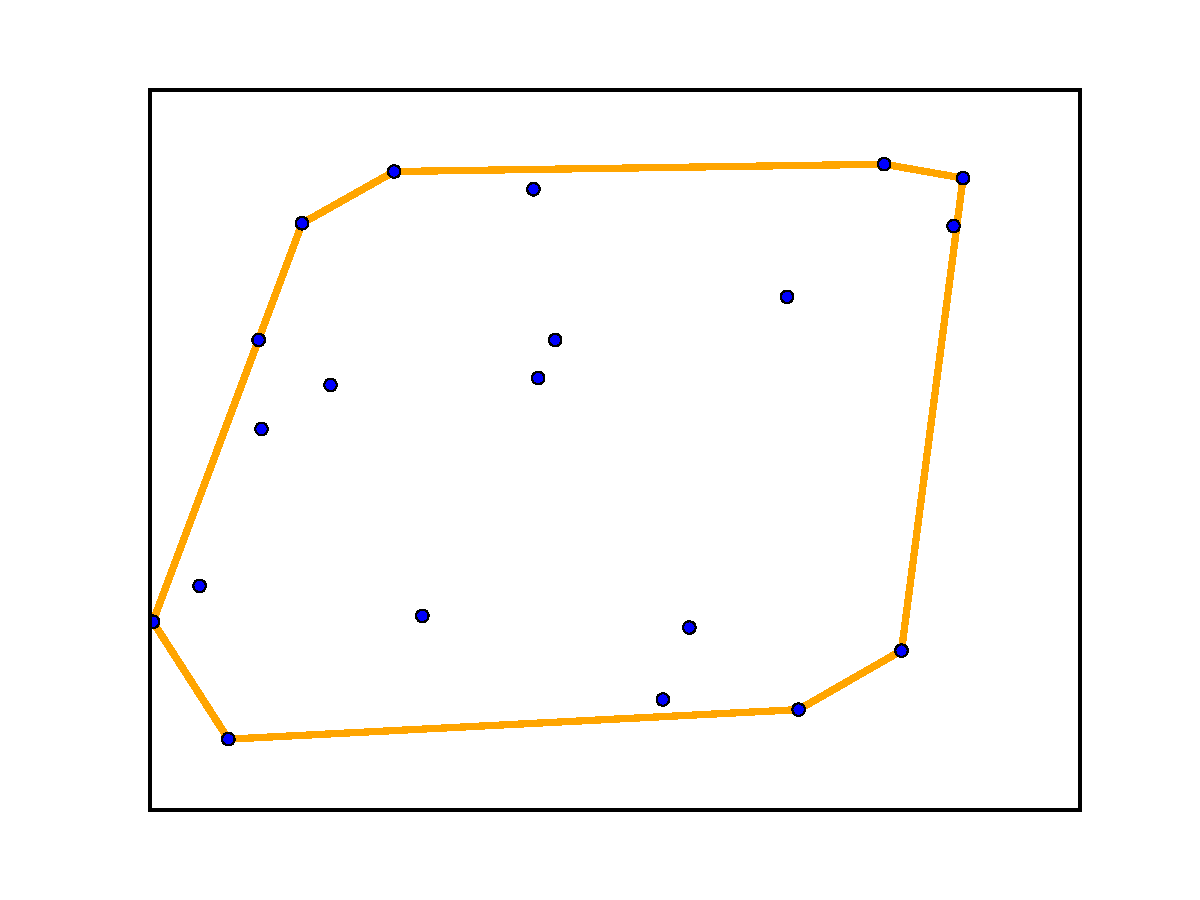
\includegraphics[width=0.49\textwidth]{chapter7/plots/qhull_final.pdf} 
   \caption{example caption}
   \label{fig:example}
\end{figure}
As an initial input we have N data points. The first operation is finding the two extreme points in the horizontal axis, which are guaranteed to be part of the convex hull. 
We connect these two extreme points thus creating a division between the left and right point set. Now the divide and conquer method begins. We will only describe what happens to the right side, but imply that the same steps are taken on the left side. 
We find the point furthest away from the dividing line and add it. This forms a triangle with all points inside the triangle not belonging to the convex hull and thus excluding them. The triangle again divides the remaining points into two sets, one left of the triangle and one right which are again iterated over recursively. 

The method is repeated until each subset only contains the start and end point of the dividing line. 
We have created the convex hull, which if projected to an d-1 dimensional space provides the \deltri\ of the projected points.



\section{Barycentric coordinates system}

For the next steps which include containing-triangle finding and interpolation we will need to introduce the barycentric coordinate system of a triangle.
One can construct the barycenter of a triangle by drawing lines from each point to the midpoint of the opposing side (see Figure \ref{fig:tri_barycenter}). 


\begin{figure}[htbp] %  figure placement: here, top, bottom, or page
   \centering
   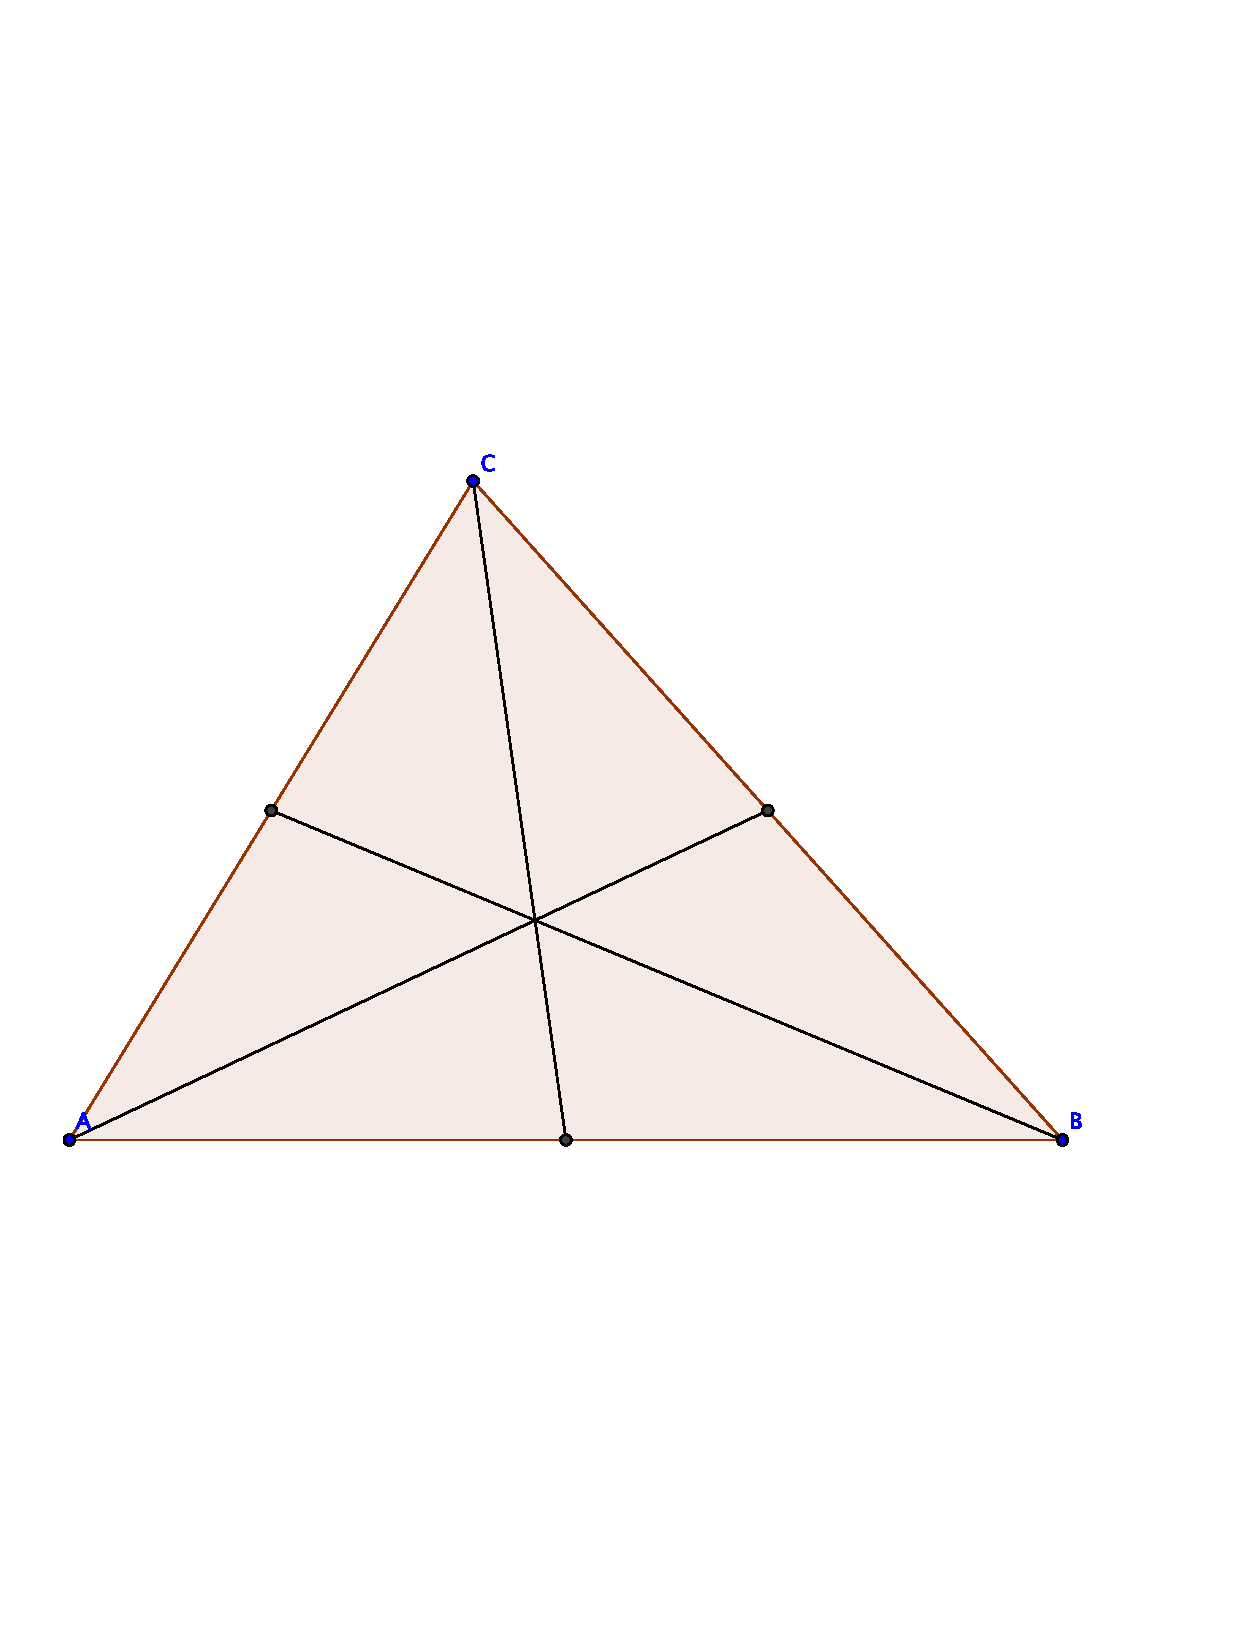
\includegraphics[width=0.7\textwidth]{chapter7/plots/barycenter.pdf}
   \caption{example caption}
   \label{fig:example}
\end{figure}


The coordinates of the barycenter M can simply be expressed by,
\[
\vec{M} = \frac{1}{3} (\vec{A} + \vec{B} + \vec{C}).
\]

Not only the barycenter can be expressed by the vectors of $\vec{A}$, $\vec{B}$ and $\vec{C}$ but every point p inside the triangle can be expressed by,
\[
\vec{p} = \alpha\vec{A} + \beta\vec{B} + \gamma\vec{C},
\]
where,
\[
\alpha + \beta + \gamma = 1
\]
. $\alpha$, $\beta$ and $\gamma$ are called the barycentric coordinates. If the point p lies within the triangle all barycentric coordinates are positive. 

\section{Triangle Finding and Interpolation}

For now we have constructed a \deltri\ of our set. We are given a point at which to interpolate. The first step is to find the triangle that contains the point by a method called directed walk (priv. comm. Pauli Virtanen). We choose a random starting triangle and calculate the barycentric coordinates for it and test if they are larger than 0. If all of them are larger than 0 we have found the containing Triangle. If the n-th (0,1 or 2 for two dimensions) barycentric coordinate is negative we find jump to the neighbour which is opposite the n-th point. This is iterated until the containing Triangle is found or the next jump would lead outside the convex hull. For the latter the point is outside of grid and can not be interpolated.

Once we find the triangle that contains the point p and we know the barycentric coordinates we can simply interpolate the function at the point by,
\[
f(\vec{p})=\alpha f(\vec{A}) + \beta f(\vec{B}) + \gamma f(\vec{C})
\]
where  $\vec{A}$, $\vec{B}$ and $\vec{C}$ are the points of the triangle. 

For now we have described everything in two dimensions, but the method is extensible to N-dimensions. The triangles (3-simplex) become n-simplices (e.g. Tetrahedron in 3 dimensions), but the method of calculating the \deltri, finding the containing simplex and interpolating remains the same.

\section{Conclusion}

don't know yet 


